\section{Kết quả mô phỏng}

Kết quả huấn luyện mô hình học sâu cho ước lượng kênh truyền vô tuyến sau 10 epochs:

\begin{lstlisting}
Epoch 1: val_loss improved from inf to 0.06108, saving model to trained_nets/SRCNN_check.keras 
Epoch 2: val_loss improved from 0.06108 to 0.05603, saving model to trained_nets/SRCNN_check.keras 
Epoch 3: val_loss improved from 0.05603 to 0.05343, saving model to trained_nets/SRCNN_check.keras 
Epoch 4: val_loss improved from 0.05343 to 0.05330, saving model to trained_nets/SRCNN_check.keras 
Epoch 5: val_loss improved from 0.05330 to 0.05226, saving model to trained_nets/SRCNN_check.keras 
Epoch 6: val_loss improved from 0.05226 to 0.05114, saving model to trained_nets/SRCNN_check.keras 
Epoch 7: val_loss improved from 0.05114 to 0.04993, saving model to trained_nets/SRCNN_check.keras 
Epoch 8: val_loss improved from 0.04993 to 0.04937, saving model to trained_nets/SRCNN_check.keras 
Epoch 9: val_loss improved from 0.04937 to 0.04879, saving model to trained_nets/SRCNN_check.keras 
Epoch 10: val_loss improved from 0.04879 to 0.04877, saving model to trained_nets/SRCNN_check.keras    
\end{lstlisting}

Đáp ứng yêu cầu về độ chính xác, mô hình đã học tốt. 
Để kiểm tra hiệu suất của mô hình, nhóm bài tập lớn sử dụng tập dữ liệu kiểm tra để đánh giá mô hình. 
Kết quả đánh giá mô hình trên tập dữ liệu kiểm tra:

\begin{figure}[H]
    \centering
    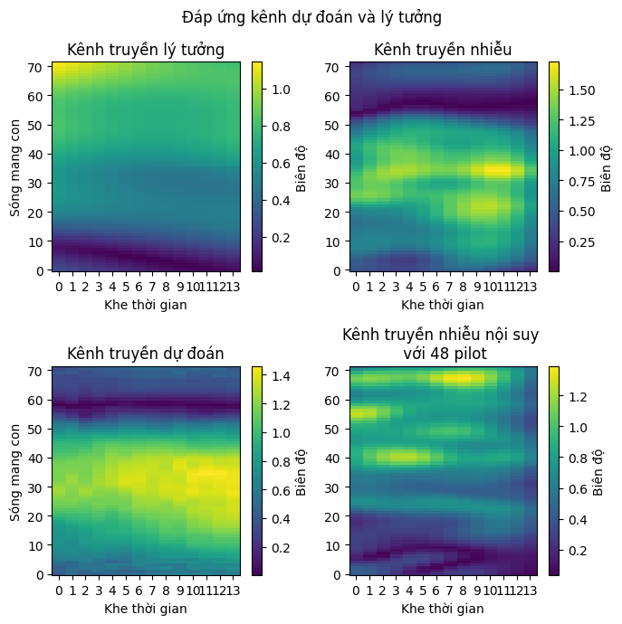
\includegraphics[width=0.75\textwidth]{../images/pred_vs_ideal.png}
    \caption{Đáp ứng kênh truyền dự đoán so với kênh truyền lý tưởng}
\end{figure}

\subsection*{Huấn luyện mô hình với số lượng pilot khác nhau}

Nhóm thực hiện huấn luyện mô hình với số lượng pilot khác nhau để xem xét hiệu suất của mô hình. 
Số lượng pilot ảnh hưởng đến dữ liệu nội suy kênh nhiễu, mà kênh nhiễu là ngõ vào của mô hình. 
Do đó, ứng với mỗi số lượng pilot, mô hình sẽ học một cách khác nhau với tập dữ liệu nội suy kênh nhiễu khác nhau.
Số lượng pilot được chọn đại diện từ tập $\{8, 16, 24, 36, 48\}$.

\begin{figure}[H]
    \centering
    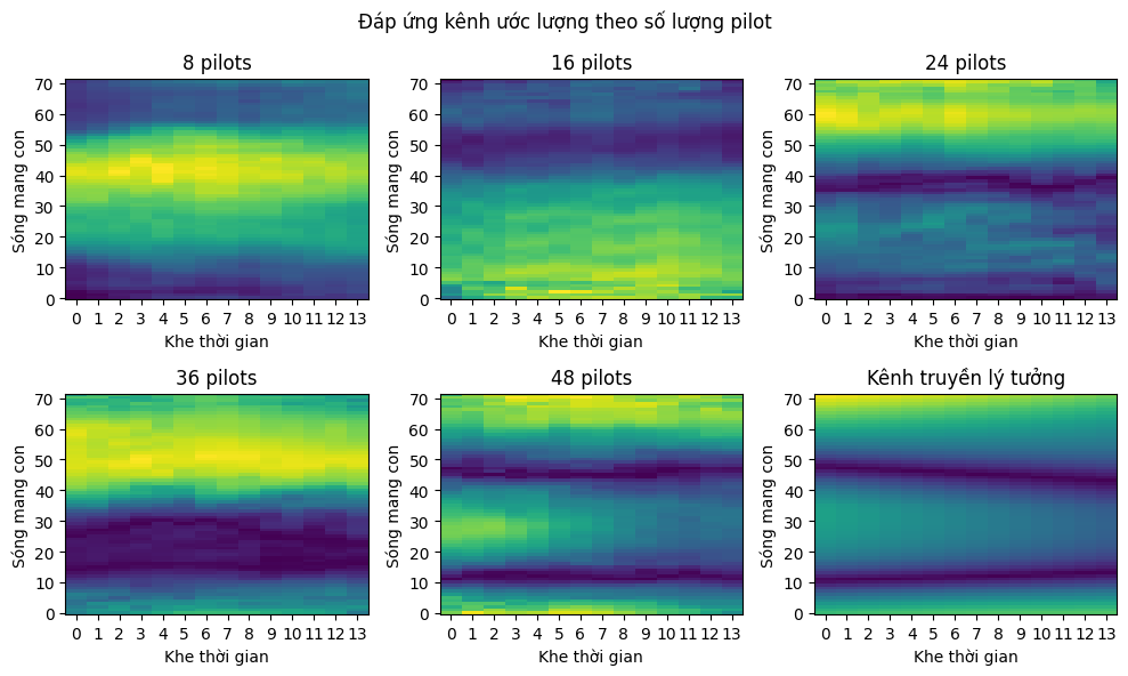
\includegraphics[width=\textwidth]{../images/channel_estimation_vs_num_pilots.png}
    \caption{Đáp ứng kênh truyền ước lượng theo số lượng pilot khác nhau}
\end{figure}

Tại SNR = 12 dB, với số lượng pilot càng nhiều thì sai số bình phương trung bình giảm dần:

\begin{figure}[H]
    \centering
    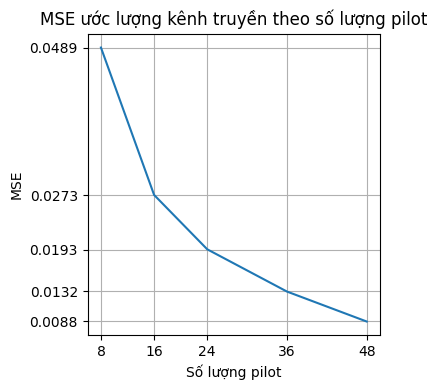
\includegraphics[width=.5\textwidth]{../images/mse_vs_num_pilots.png}
    \caption{Sai số bình phương trung bình giảm dần theo số lượng pilot}
\end{figure}